\documentclass[nooutcomes]{ximera}


\newcommand{\RR}{\mathbb R}
\renewcommand{\d}{\,d}
\newcommand{\dd}[2][]{\frac{d #1}{d #2}}
\renewcommand{\l}{\ell}
\newcommand{\ddx}{\frac{d}{dx}}
\newcommand{\dfn}{\textbf}
\newcommand{\eval}[1]{\bigg[ #1 \bigg]}

\usepackage{multicol}

\renewenvironment{freeResponse}{
\ifhandout\setbox0\vbox\bgroup\else
\begin{trivlist}\item[\hskip \labelsep\bfseries Solution:\hspace{2ex}]
\fi}
{\ifhandout\egroup\else
\end{trivlist}
\fi}
\usepackage{fullpage}

\title{Briggs 5.4: Working with Integrals}

\begin{document}
\begin{abstract}
\end{abstract}
\maketitle


%problem 1
\begin{problem}

  \begin{enumerate}
    \item
    If $f$ is an odd function, why is it true that $\int_{-a}^a f(x)
    \d x = 0$?  
    Support your reasoning with a picture.
    \begin{freeResponse}
      If $f$ is odd, then the regions between the graph of $f$ and the $x$-axis from $[-a,0]$ and $[0,a]$ are reflections of each other through the origin.
      Thus, these two regions will have the same area but with opposite signs since they are on opposite sides of the $x$-axis.
      They will therefore cancel each other out.
		
      \begin{image}
        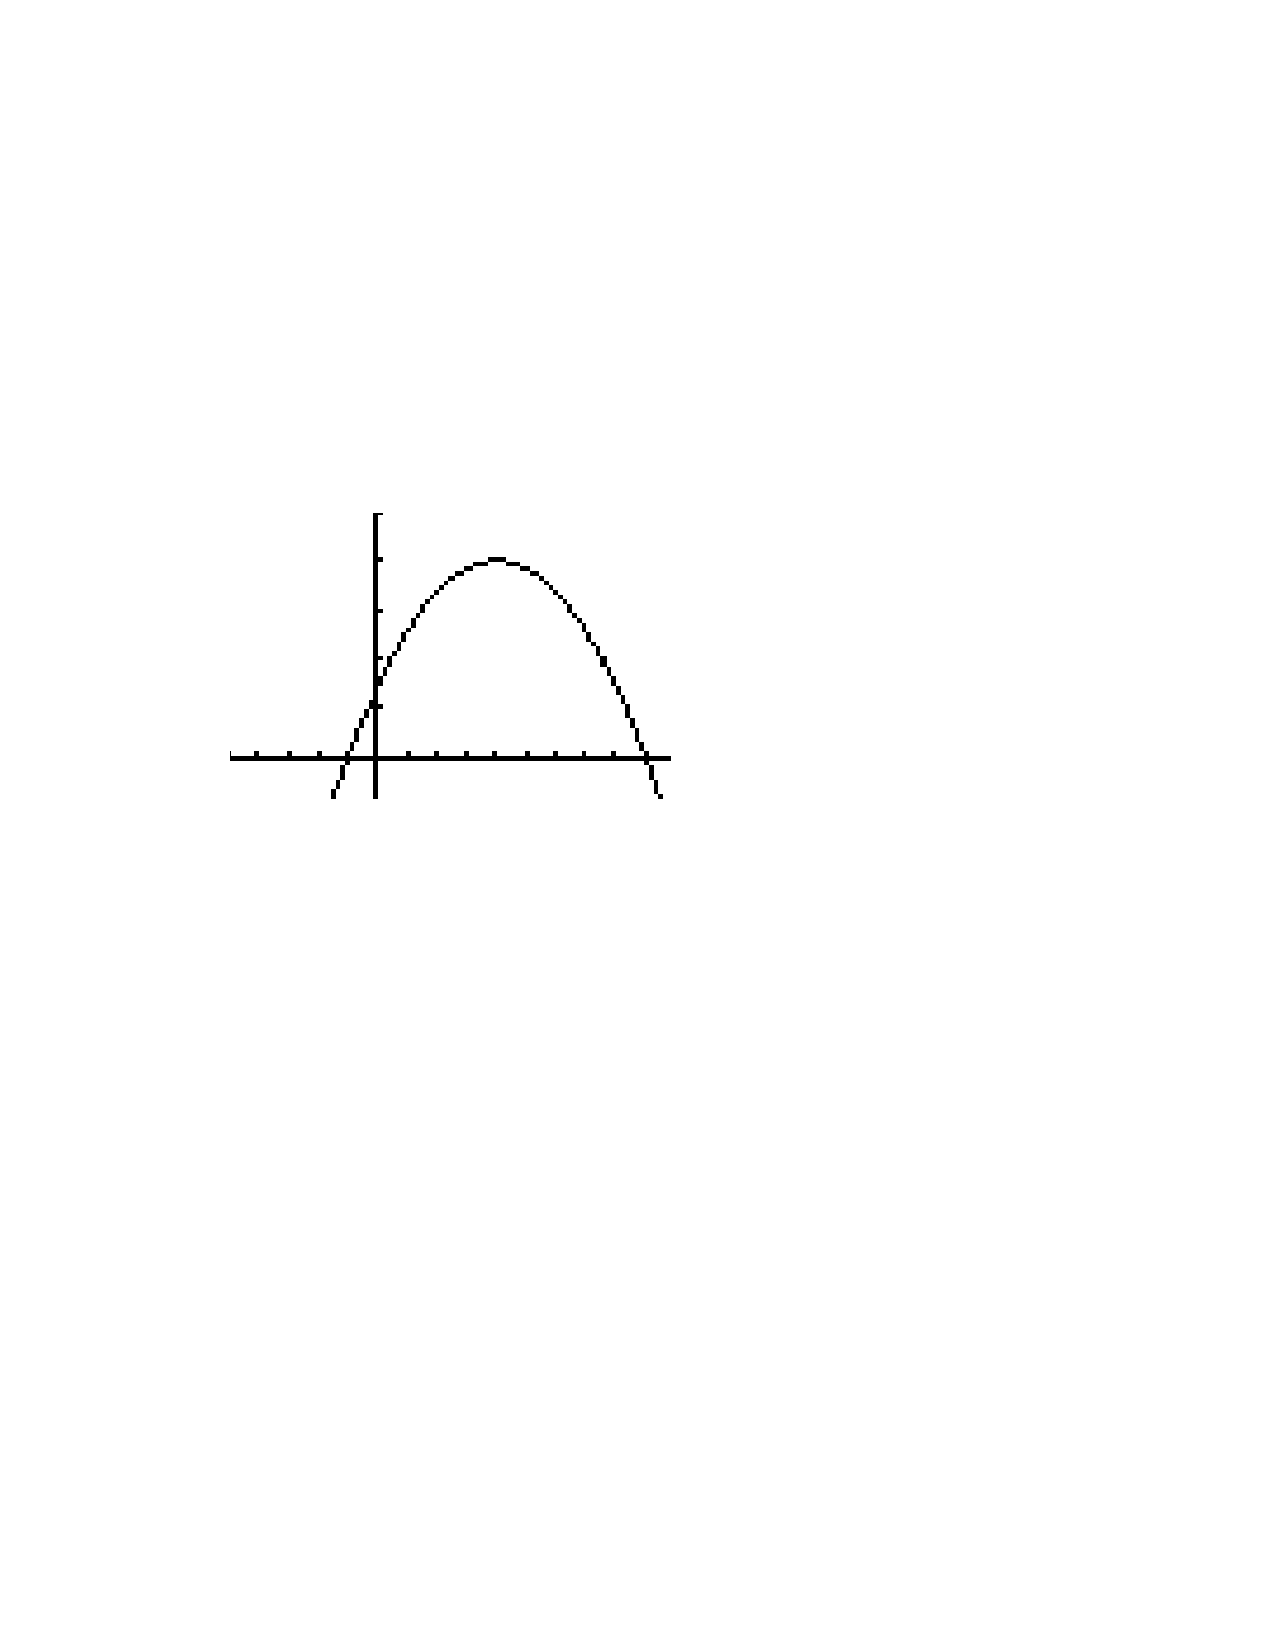
\includegraphics[scale=.7]{Images/Figure1.png}
      \end{image}
    \end{freeResponse}
		
    \item
      If $f$ is an even function, why is it true that $\int_{-a}^a f(x) \d x = 2 \int_0^a f(x) \d x$?
      Support your reasoning with a picture.
      \begin{freeResponse}
        If $f$ is even, then the regions between the graph of $f$ and the $x$-axis from $[-a,0]$ and $[0,a]$ are reflections of each other through the $y$-axis.
        Thus, these two regions will have the same area with the same sign since they are on the same sides of the $x$-axis.
        So you can only find one of these areas and then double it.
      \begin{image}
        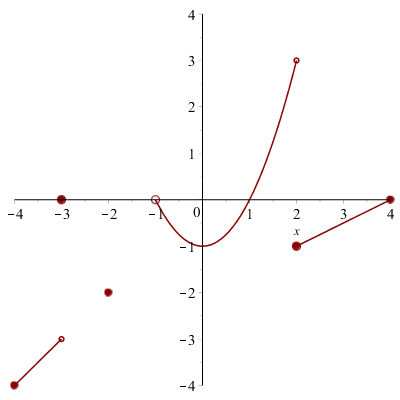
\includegraphics[scale=.7]{Images/Figure2.png}
      \end{image}
    \end{freeResponse}
    \end{enumerate}
\end{problem}

%problem 2
\begin{problem}

  \begin{enumerate}
    \item
      Find the following definite integral:
	\begin{equation*}
          \int_{-4}^4 \frac{x^2 \sin^3(x)}{\sqrt{x^4 + 1}} \d x
	\end{equation*}
	\begin{freeResponse}
          Let $f(x) = \frac{x^2 \sin^3(x)}{\sqrt{x^4 + 1}}$.  
	  Then notice that
          \begin{align*}
            f(-x) &= \frac{(-x)^2 \sin^3(-x)}{\sqrt{(-x)^4 + 1}}  \\
                  &= \frac{x^2 (- \sin(x))^3}{\sqrt{x^4 + 1}}  \quad \text{(since } \sin(x) \text{ is an odd function)}  \\
                  &= \frac{- x^2 \sin^3(x)}{\sqrt{x^4 + 1}}  \\
                  &= -f(x).
          \end{align*}
          Thus, $f$ is an odd function and therefore
          \begin{equation*}
            \int_{-4}^4 \frac{x^2 \sin^3(x)}{\sqrt{x^4 + 1}} \d x = 0.
          \end{equation*}
	\end{freeResponse}
		
	\item
          Suppose that $f$ is an even function.
          Given that $\int_0^6 f(x) \d x = 13$, find $\int_{-6}^6 (5f(x) + 14) \d x$.
          \begin{freeResponse}
            First notice that
            \begin{equation}\label{linear integral}
              \int_{-6}^6 (5f(x) + 14) \d x = 5 \int_{-6}^6 f(x) \d x + \int_{-6}^6 14 \d x.
            \end{equation}
            
            Since $f$ is even, we know that
            \begin{equation}\label{int of f}
              \int_{-6}^6 f(x) \d x = 2 \int_0^6 f(x) \d x = 2 (13) = 26.
            \end{equation}
            
            We also know that $g(x)=14$ is also an even function.  We have:
             $\int_{-6}^6 14 \d x = 2\int_{0}^6 14 \d x$
            \begin{equation}\label{int of 14}
              2\int_{0}^6 14 \d x = \eval{14x}_{0}^6 = 2(14)(6) = 168.
            \end{equation}
            
            Then substituting equations \eqref{int of f} and \eqref{int of 14} into equation \eqref{linear integral} gives:
            \begin{equation*}
              \int_{-6}^6 (5f(x) + 14) \d x = 5(26) + 168 = 130 + 168 = 298.
            \end{equation*}
          \end{freeResponse}
	\end{enumerate}
\end{problem}

%problem 3
\begin{problem}
Evaluate the following integrals using symmetry arguments.

\begin{enumerate}

   \item    $\int_{-\pi/4}^{\pi/2} \sin(t) \d t$

      \begin{freeResponse}
        Since the function $f(t) = \sin(t)$ is odd, we will break the interval into $[-\pi/4, \pi/4]$ and $[\pi/4,\pi/2]$
        \begin{align*}
        \int_{-\pi/4}^{\pi/2} \sin(t) \d t&= \int_{-\pi/4}^{\pi/4} \sin(t) \d t + \int_{\pi/4}^{\pi/2} \sin(t) \d t\\
        &=0+\eval{(-\cos(t))}_{\pi/4}^{\pi/2}\\
	&=-\cos(\pi/2)-(-\cos(\pi/4))\\
	&=\cos(\pi/4)\\
	&=\sqrt{2}/2   
        \end{align*}
      \end{freeResponse}
      
      \item $\int_{-2}^2 (1+x+3x^2-x^9) \d x$
      \begin{freeResponse}
	In order to take advantage of symmetry, we will split the given polynomial into a sum of its even and odd parts.  We will then integrate each part separately:
        $$\int_{-2}^2 (1+x+3x^2-x^9) \d x= \int_{-2}^{2} (1+3x^2) \d x + \int_{-2}^{2} (x-x^9) \d x$$
        
        We will first integrate an even function:\\
$\int_{-2}^{2} (1+3x^2) \d x =2\int_{0}^{2} (1+3x^2) \d x=2\eval{x+x^3}_0^2=2(2+8)=20$

Then an odd function:\\
$\int_{-2}^{2} (x-x^9) \d x=0$

Therefore:$\int_{-2}^2 (1+x+3x^2-x^9) \d x=20$
      \end{freeResponse}
      
      \item
     $\int_0^{\pi} \cos(x) \d x$ 
      \begin{freeResponse}
        Over the interval $[0, \pi]$ the curve $y = \cos(x)$ is symmetric about the point $(\pi/2,0)$. 
        \begin{image}
          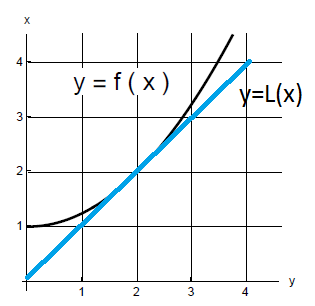
\includegraphics[scale = 0.6]{Images/figure4.png}
        \end{image}
        That means that the graph of the function on the interval $[0,\pi/2]$, you can obtain the entire graph by simply rotating through $180^{\circ}$ about the point $(\pi/2,0)$.  From the graph above, we can see that the net area of the region between the curve $y=\cos(x)$ and the $x$-axis is $0$.   
        Therefore, $\int_0^\pi \cos(x) \d x =0$
      \end{freeResponse}
      
      
\end{enumerate}
\end{problem}

%problem 4
\begin{problem}

      A cup of coffee has temperature $20 + 75e^{-.02t}$ degrees (Celsius) $t$ minutes after being poured into a cup.  
      What is the average temperature of the coffee during the first half hour?
      \begin{freeResponse}
        Let $T(t) := 20 + 75e^{-.02t}$.  We want the average value of $T$ on $[0,30]$.
        \begin{align*}
          T_{\text{avg}} &= \frac{1}{30-0} \int_0^{30} \left( 20 + 75e^{-.02t} \right) \d t  \\
                         &= \frac{1}{30} \eval{20t - \frac{75}{.02} e^{-.02t}}_0^{30}  \\
                         &= \frac{1}{30} \eval{20t - 3750 e^{-.02t}}_0^{30}  \\
                         &= \frac{1}{30} \left[ \left( 20(30) - 3750e^{-0.6} \right) - (0 - 3750) \right]  \\
                         &= \frac{1}{30} \left( 4350 - 3750e^{-0.6} \right)  \\
                         &= 145 - 125e^{-0.6} 
        \end{align*}
        So the average temperature of the coffee during the half hour is $145 - 125e^{-0.6} \approx 76.4$ degrees Celsius.
      \end{freeResponse}
    

\end{problem}


%problem 5
\begin{problem}
 The graph of a function $f$ defined on the interval $[0,6]$  is given in the figure.
  
        \begin{image}
          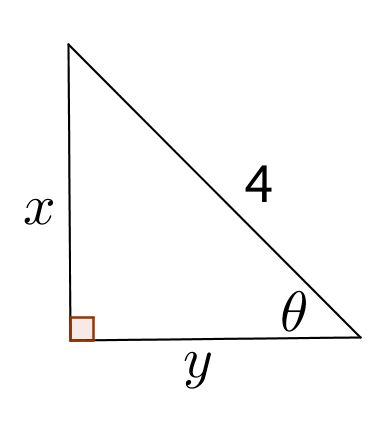
\includegraphics[scale = 0.6]{Images/figure5.png}
        \end{image}
     \begin{enumerate}
     \item Compute the net area of the region between the graph of $f$ and the $x$-axis, on the interval $[0,6]$.
     \begin{freeResponse}
     The net area $= -1/2 + 1/2 +1 +3+1=5$
     \end{freeResponse}
        
     \item Draw a rectangle with base on the $x$-axis, $0\leq x \leq 6$, whose area is equal to the net area in part (a).
     \begin{freeResponse}
     Let $A$ be the area of the rectangle.  Then $A=$(base)(height)$=6h=5$.  \\
     So, $6h=5 \implies h=\frac{5}{6}$
            \begin{image}
          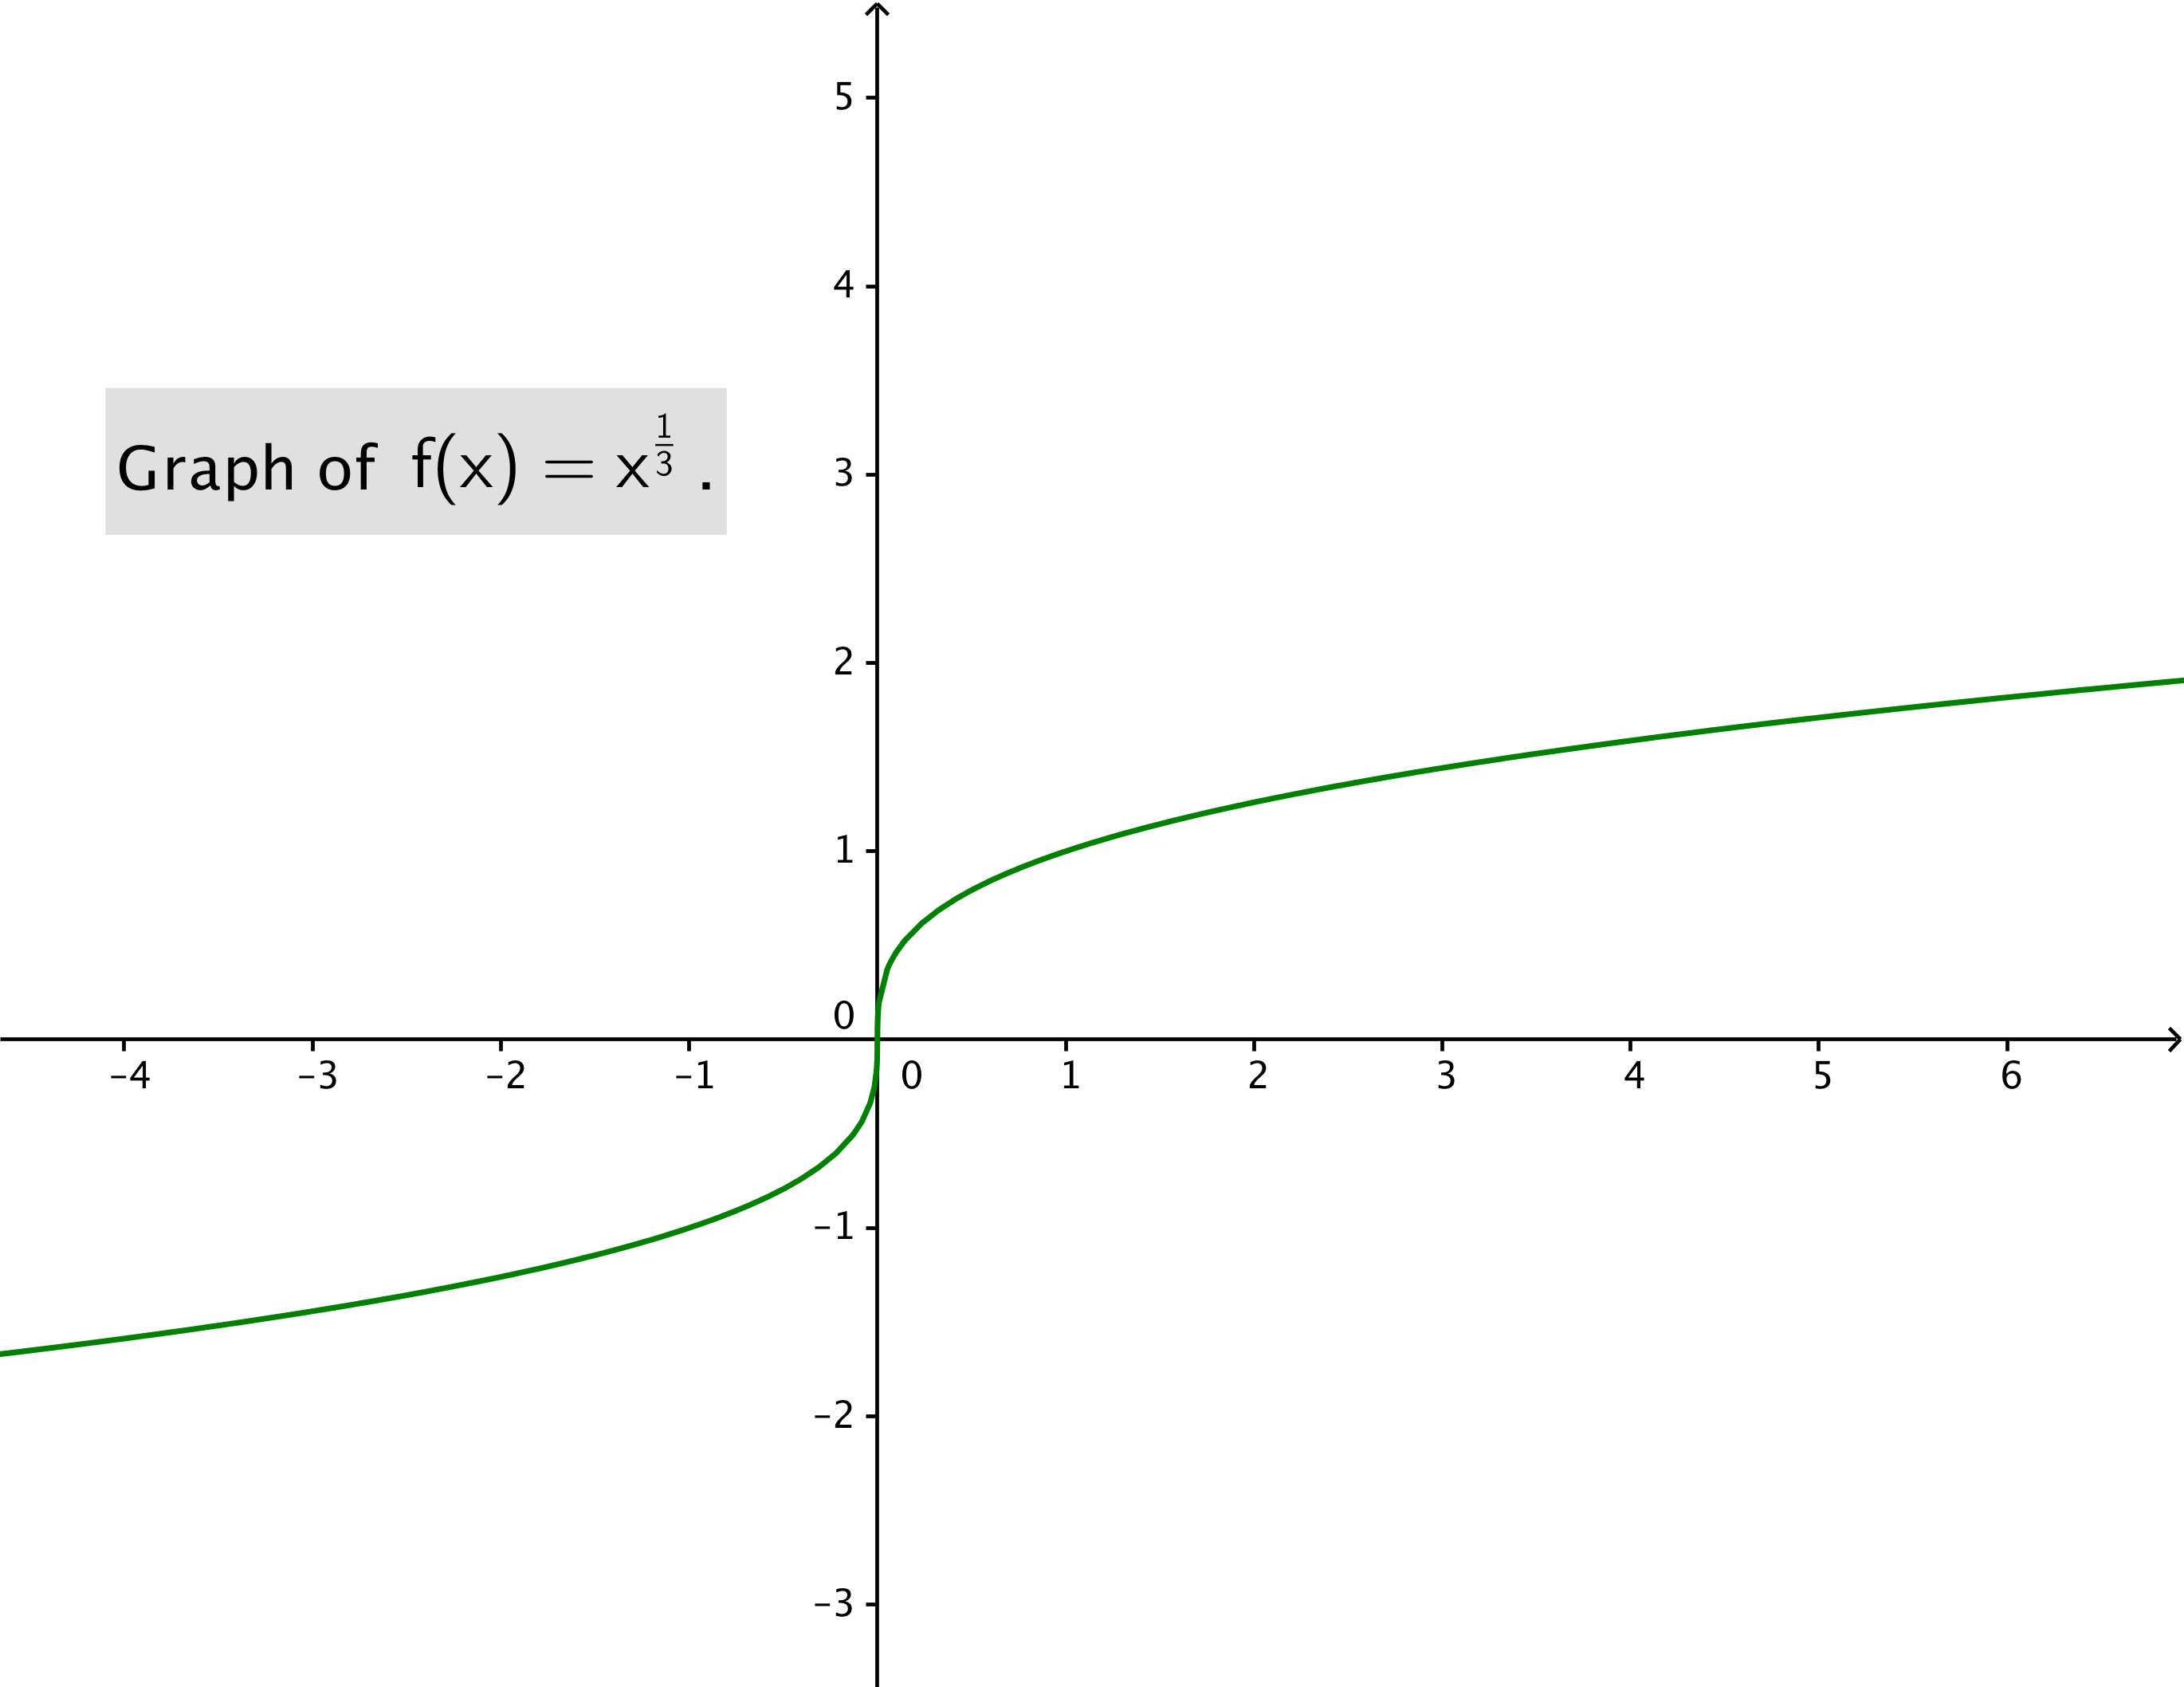
\includegraphics[scale = 0.5]{Images/figure6.png}
        \end{image}
     \end{freeResponse}
     
          \item Find a point $c$ in $(0,6)$ such that $f(c)$ is the height of the rectangle from part (b).
     \begin{freeResponse}
    $f(c)=h=\frac{5}{6}$
            \begin{image}
          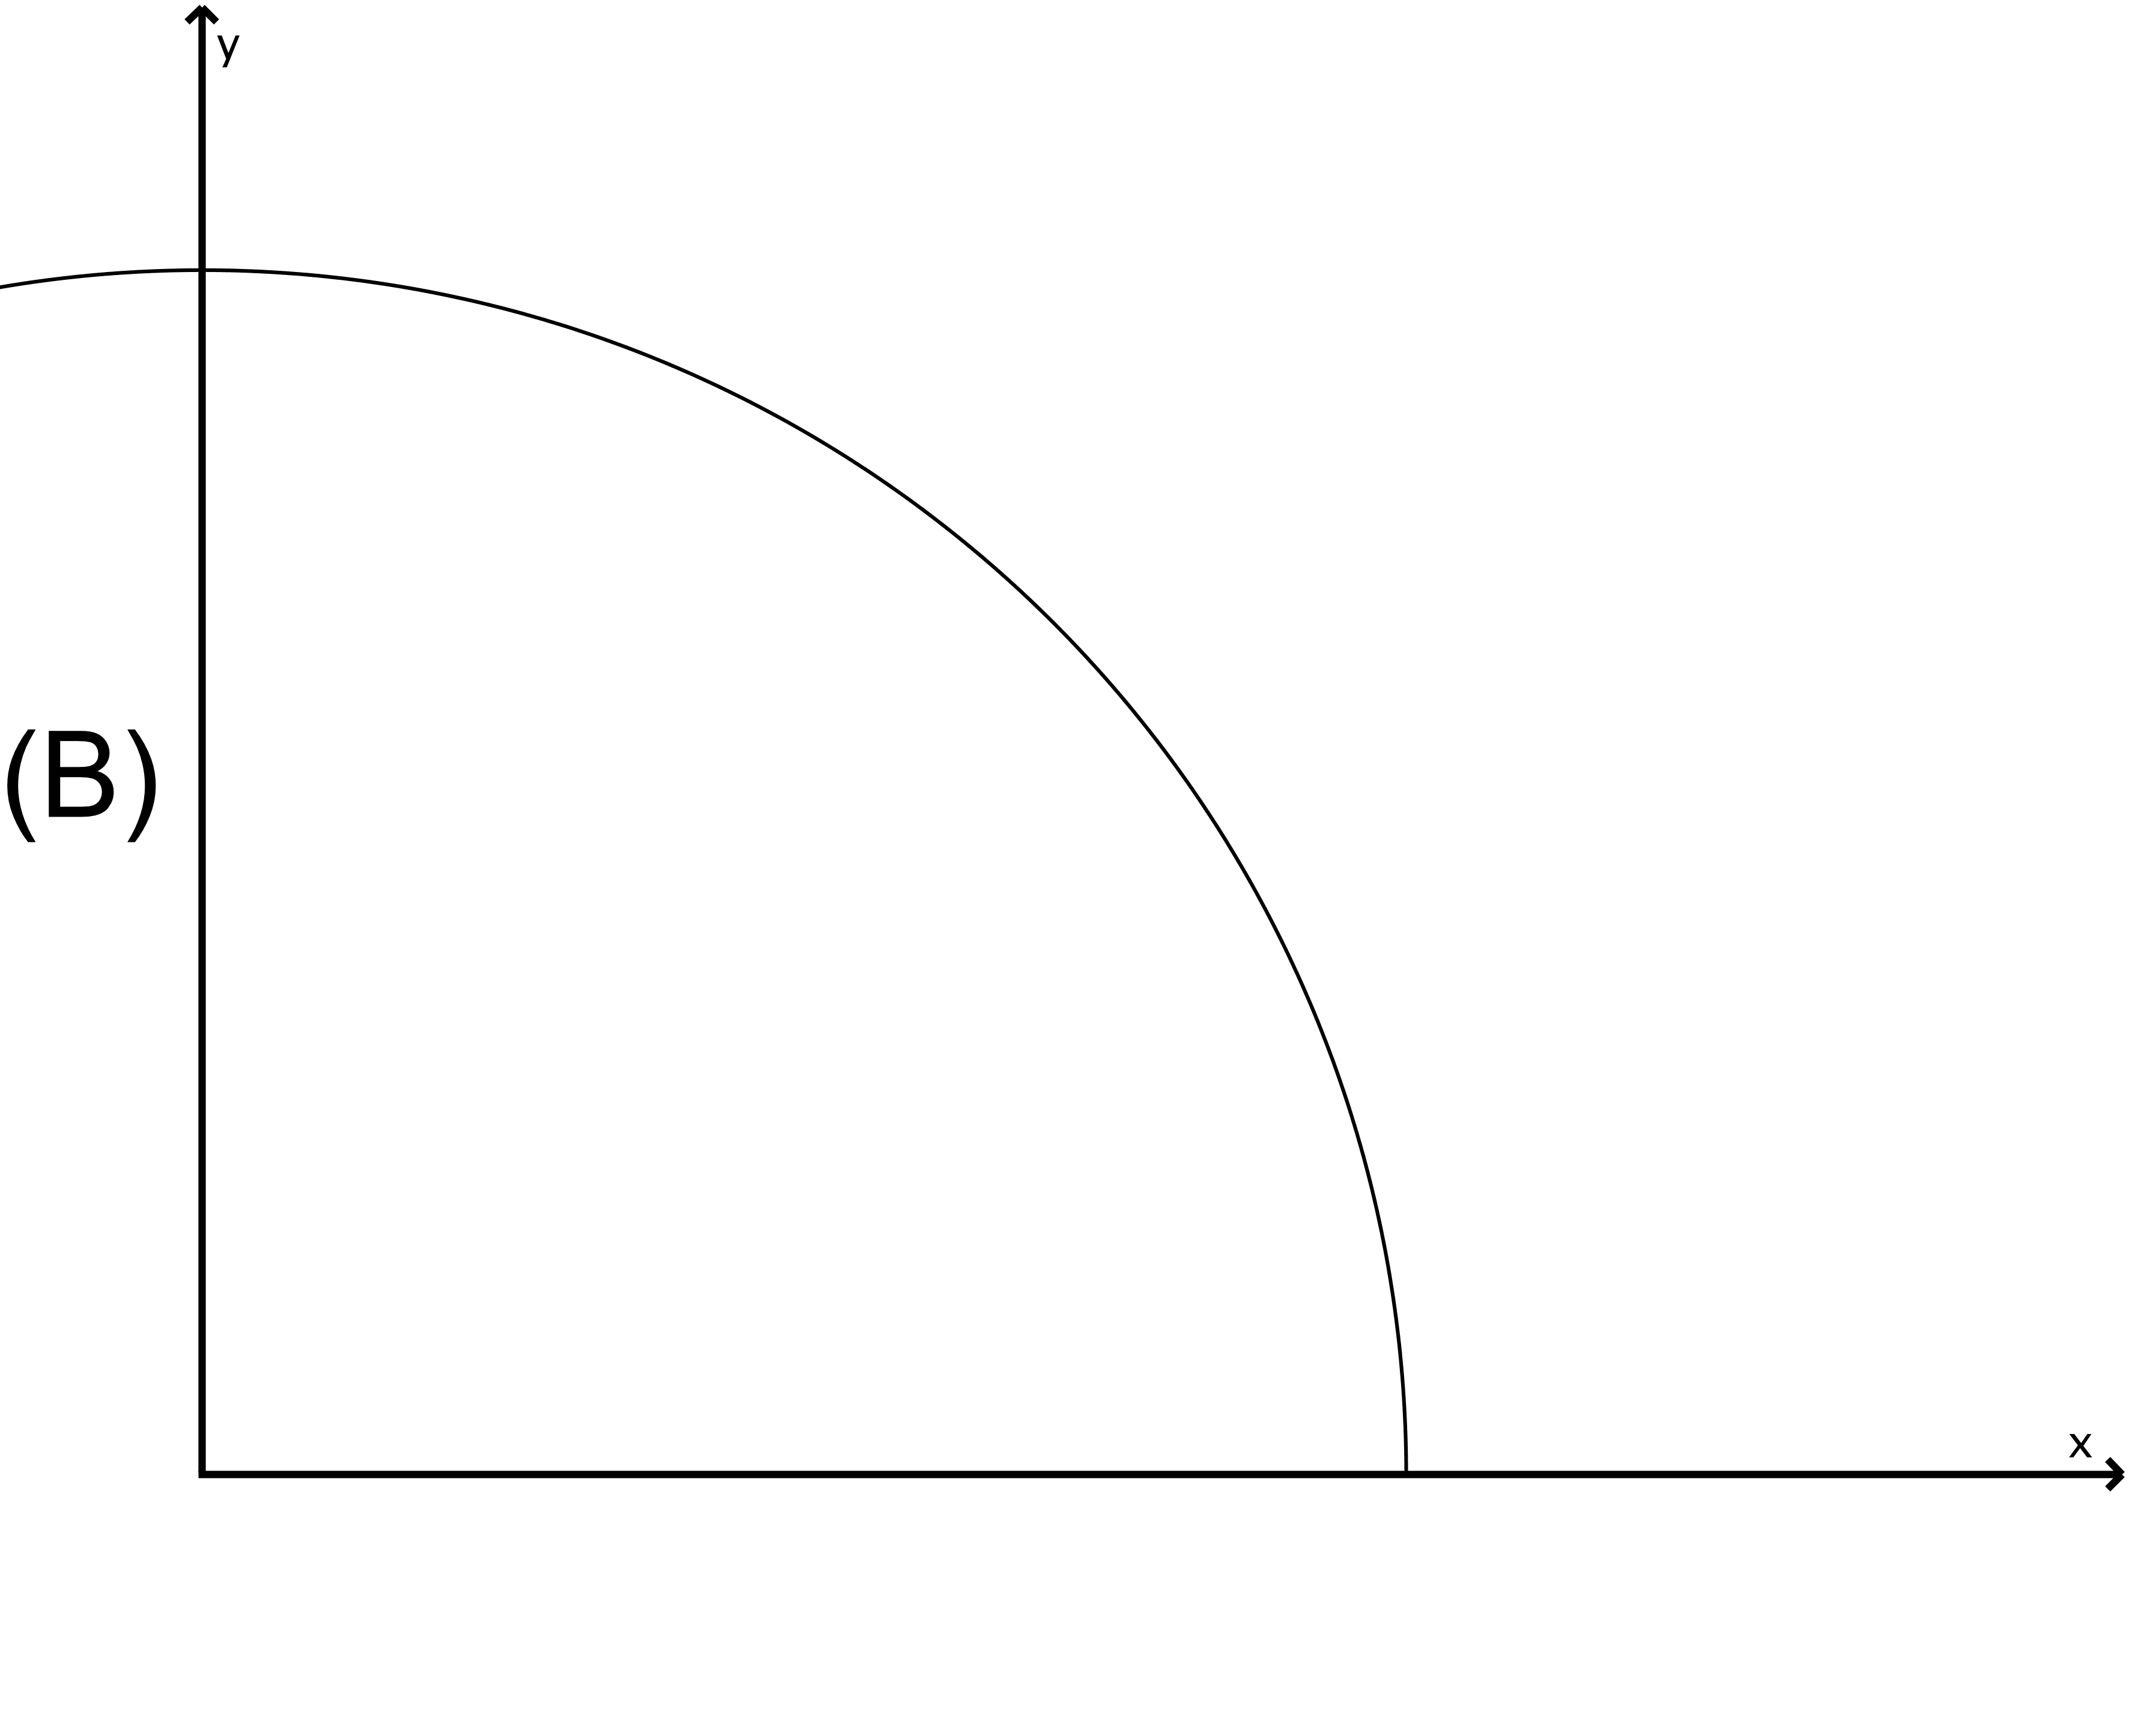
\includegraphics[scale = 0.5]{Images/figure7.png}
        \end{image}
     \end{freeResponse}
     \item
           Using the figure and parts (a-c), what is the relationship between the rectangle from part (b), the net area from part (a), and the average value of $f$ on $[0, 6]$?
      \begin{freeResponse}
        The Mean Value Theorem for integrals states that there exists a point $d$ in $(a, b)$ such that
        \[
          f(d) = \frac{1}{b-a}\int_a^b f(x) \d x.
        \]
        The right-hand side of this equation is the average value of $f$ on $[a, b]$.

        Rewriting we have
        \[
        f(d) \cdot (b-a) = \int_a^b f(x) \d x.
        \]
      The right-hand side of this equation is the area under the curve $y = f(x)$, found in part (a): $\int_0^6 f(x) \d x=5$.\\
       The left-hand side of this equation is the area of the rectangle in part (b).  The point $d$ in the general MVT for integrals forumula is the point $c$ we found in part (c).  From (b) and (c), $f(c)=\frac{5}{6}$ so the left-hand side of this equation is:  $\frac{5}{6} \cdot [6-0]=5$ 
        \end{freeResponse}
     \end{enumerate}
     \end{problem}

%problem 6
\begin{problem}

  Find all points at which the given function equals its average value on the given interval.
  \begin{enumerate}
    \item
      $f(x) = e^x	\qquad	[0,4]$
      \begin{freeResponse}
        First, we need to find $f_{\text{avg}}$:
        \begin{align*}
          f_{\text{avg}} &= \frac{1}{4-0} \int_0^4 e^x \d x  \\
                         &= \frac{1}{4} \eval{e^x}_0^4  \\
                         &= \frac{1}{4} \left( e^4 - 1 \right)  
        \end{align*}
        So we are looking for all values $c \in [0,4]$ such that:
        \begin{align*}
          f(c) &= \frac{1}{4} (e^4 - 1)  \\
          \Longrightarrow \quad e^c &= \frac{1}{4} (e^4 - 1)  \\
          \Longrightarrow \quad c &= \ln \left( \frac{1}{4} (e^4 - 1) \right)
        \end{align*}
        Therefore, our answer is $\ln \left( \frac{1}{4} (e^4 - 1) \right)$.
      \end{freeResponse}

    \item
      $g(x) = \frac{\pi}{4} \sin(x)	\qquad	[0,\pi]$
      \begin{freeResponse}
        First, we need to find $g_{\text{avg}}$:
        \begin{align*}
          g_{\text{avg}} &= \frac{1}{\pi-0} \int_0^{\pi} \frac{\pi}{4} \sin(x) \d x  \\
                         &= \frac{1}{4} \eval{-\cos(x)}_0^{\pi}  \\
                         &= \frac{1}{4} \left( - (-1-1) \right)  \\
                         &= \frac{1}{2}
        \end{align*}
        So we are looking for all values $c \in [0,\pi]$ such that:
        \begin{align*}
          &g(c) = \frac{1}{2}  \\
          &\Longrightarrow \quad \frac{\pi}{4} \sin(c) = \frac{1}{2}  \\
          &\Longrightarrow \quad \sin(c) = \frac{2}{\pi}  \\
          &\Longrightarrow \quad c = \arcsin \left( \frac{2}{\pi} \right), \pi - \arcsin \left( \frac{2}{\pi} \right)
          &\end{align*}
        Therefore, our two answers are $\arcsin \left( \frac{2}{\pi} \right), \pi - \arcsin \left( \frac{2}{\pi} \right)$.
    \end{freeResponse}
  \end{enumerate}
\end{problem}


\end{document} 
